\documentclass[letter]{article}
\usepackage{amsmath}
\usepackage{amsfonts}
\usepackage{amssymb}
\usepackage{ifthen}
\usepackage{fancyhdr}
\usepackage{graphicx}
\usepackage{subcaption}
\usepackage[shortlabels]{enumitem}

\newcommand{\fref}[1]{\textbf{Figure \ref{#1}}}

%%%
% Set up the margins to use a fairly large area of the page
%%%
\oddsidemargin=.2in
\evensidemargin=.2in
\textwidth=6in
\topmargin=0in
\textheight=9.0in
\parskip=.07in
\parindent=0in
\pagestyle{fancy}

%%%
% Set up the header
%%%
\newcommand{\setheader}[6]{
	\lhead{{\sc #1} {\sc #2}\\{} ({\small \it \today})}
	\rhead{
		{\bf #3} 
		\ifthenelse{\equal{#4}{}}{}{(#4)}\\
		{\bf #5}
		\ifthenelse{\equal{#6}{}}{}{(#6)}%
	}
}

\begin{document}
	\setheader{CSC490}{Module 1}{Ben Weisz}{}{Qiwen Hua}{}

	\section{Focal Loss \& Anisotropic Guassian}

	\subsection{Motivation}

	\subsection{Techniques}

	\subsection{Evaluation}

	\subsection{Limitations}

	\section{Multi-class Detector}

    In this section, we will discuss details regarding extending our detector system to detect more than one class of objects (cars in Part A). 

	\subsection{Motivation}

    After finishing Part A of this module, our detector possesses the ability to detect cars with LiDAR point clouds. However, in the real world applications of self driving car perceptions, detecting only one class is insufficient, as there are many more important classes of objects surrounding the car: pedestrians, signs, bicycles, signals, etc. 
    
    This problem is relevant as the number of classes of objects our system can detect is directly related with how well our system perceives the world. In other word, tackling this problem directly improves the safety and practicality of our detector system. 

    We choose to move forward with this idea as we not only want our detector system to be accurate but also to be well-rounded. Having our system to be able to detect multiple classes makes it more functional in the real world. 

	\subsection{Techniques}

    Naturally, the traits (e.g., sizes, average movement speeds, frequently appearing locations) of each classes of objects different wildly. For example, the BEV sizes of vehicles and pedestrians can differ by a factor of 51 ($ 1.7m \times 4.5m $ car and $ 0.5m \times 0.3m $ human). Therefore, if we want our system to be able to predict $ N_c $ object classes, our approach would be to build $ N_c $ detection models each being responsible to detect one corresponding object class. This intuition is similar to one-vs-rest classification where we use multiple binary classifications for multi-class classification. 

	Since we are building multiple single-class detection models, we do not need to modify the existing algorithm for the \verb|DetectionModelConfig| and \verb|DetectionModel| Python classes. However, we need to make changes to the following components: \begin{enumerate}
		\item \textbf{Dataset:} All entrypoints of the detector system use the \verb|pytorch|'s \verb|DataLoader| class to load the dataset of type \verb|PandasetDataset|. Therefore, to include data points from all interested classes, the first step would be to modify the \verb|PandasetDataset| class. 
		
		The \verb|__getitem__| method originally returns the BEV voxel grid tensor, the ground truth target tensor, and a set of grouud truth BEV detections of class \verb|Dectections|. While the first item (BEV voxel grid) is class independent, the latter two only describes the vehicles. We modifed the last two return types of this function to be dictionaries with the keys being the interested object classes and the values being the original ground truth target tensors and detections. 

		In addition, we need to modify the \verb|custom_collate| function slightly to be compatible with the modified \verb|__getitem__| method. 

		\item \textbf{Visualization:} We want our detection visualizations to draw detections of all interested classes in one single figure. Therefore, we updated the \verb|visualize_detections| function take in dictionaries of both detections and labels input. In the function body, we iterate through the dictionaries and use the original algorithm to plot the objects while changing the color slightly at each iteration to distinguish between the different object classes. 
		
		\item \textbf{Overfitting and training:} With all the preparations finished, we can now modify the \verb|overfit| and \verb|train| functions in \verb|main.py|. These two functions are similar as they both need to train on different classes. First, we modified the implementations to initialize models, loss functions, and optimizers for each classes and store them in three dictionaries. Then, we loop over the interested classes on top of the previous training loops and train on the corresponding class-specific models. Once an iteration finish, i.e., a single-class model has finished training, we store the model checkpoint. In the end, we will have stored $ N_c $ model checkpoints. 
		
		After the training is complete, we build a dictionary of detections by iterating over the interested classes again and use the corresponding models to make inferences. Finally, the combined detections dictionary is sent to the \verb|visualize_detections| function mentioned earlier.

		\item \textbf{Testing:} Now that we have trained our models and stored the model checkpoint for each object classes, we can test our model with \verb|test| with some modifications. First, since we have one single-class model for each object class, we need to correspondingly supply more than one model checkpoints. Our current implementation uses the substring \verb|"\\"| as seperators to pass in multiple checkpoint paths as a single string. Note that we can also pass in a single path to a file with one checkpoint path at each line; this method would be better if we have many interested object classes. 
		
		After parsing the model checkpoints and initializing the corresponding models, we loop over the interested classes and make inferences in each frame iteration. The detections for all classes are combined as discussed previously, and the system visualizes a single plot for each frame. 

	\end{enumerate}

	\subsection{Evaluation}

	Unfortunately, the number of samples are not abundant for classes other than cars in the current dataset (will be discussed more later in \S 2.4 Limitations). Therefore, we need to train the models over a large number of epochs to obtain meaningful and reasonably representative models. However, this is currently not feasible due to hardware limitations, i.e., the OS consistently sends \verb|SIGKILL| to the training process halfway due to extreme resource starvation. 

	Thus, the only way to evaluate our multi-class detector is to see the overfit result of a single frame. Here we will focus specifically at the pedestrians class. Since the pedestrian objects are much smaller than the car objects, it would naturally take more iterations for the detector to converge on the heatmap. Therefore, we set the iterations count to 1,500 and set the \verb|score_threshold| hyperparameter to -3.9 and start overfitting. Note that we have chosen frame 200 as this frame has a large number of pedestrians. 
	
	\begin{figure}[h]
		\begin{subfigure}[t]{0.49\textwidth}
			\centering
			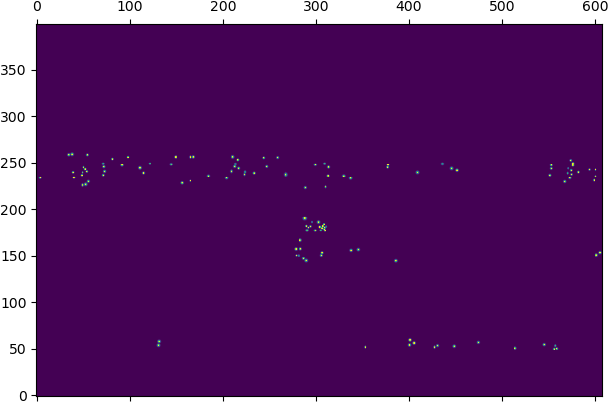
\includegraphics[width=\linewidth]{images/hm_overfit_target_pedes.png}
			\caption{Target pedestrians heatmap}
			\label{fig:hmpedes_a}
		\end{subfigure}
		\begin{subfigure}[t]{0.49\textwidth}
			\centering
			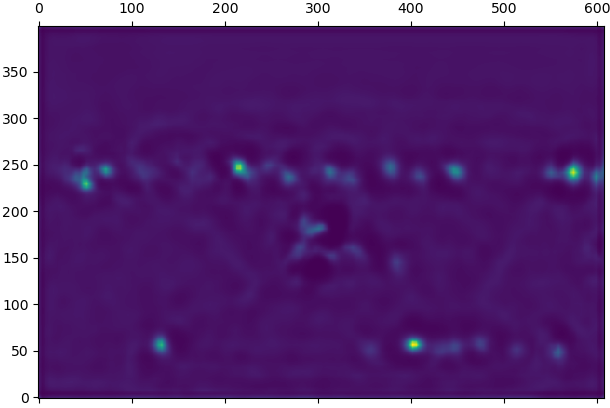
\includegraphics[width=\linewidth]{images/hm_overfit_pedes.png}
			\caption{Predicted pedestrians heatmap}
			\label{fig:hmpedes_b}
		\end{subfigure}

		\caption{Pedestrians heatmap after overfitting frame 200 of PandaSet}
		\vspace*{3mm}
	\end{figure}

	\begin{figure}[h]
		\centering
		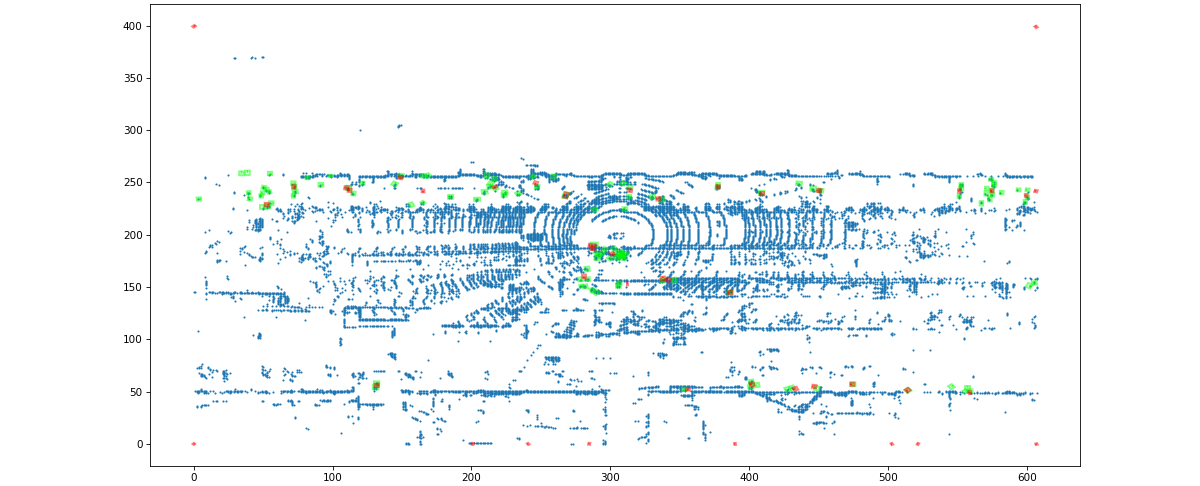
\includegraphics[width=\linewidth]{images/det_overfit_pedes.png}
		\caption{Pedestrians detections after overfitting frame 200 of PandaSet}
		\label{fig:detpedes}
	\end{figure}

	In \fref{fig:hmpedes_a} and \fref{fig:hmpedes_b}, we can see that the predicted heatmap resembles some traits of the target heatmap. However, since the pedestrians are so small in the voxel grid and are often gathered closely, the predicted heatmap can only detect the locations of clusters of pedestrians. 

	The results of the pedestrian detections are shown in \fref{fig:detpedes} with the green boxes being the ground truth labels and red boxes being the detections. As mentioned before, since our detection heatmap can only detect clusters of small objects (in this case, pedestrians), the detector only makes one detection per cluster. Thus we can see that there are only one red box for each closely positioned pedestrian groups. 

	\subsection{Limitations}

	As mentioned in \S 2.3 Evaluation, due to limited number of observations, the model performs poorly if the number of iterations (or epochs) is not large enough. In addition, the current neural network setup does not work well with small objects sizes. To better detect small objects such as pedestrians and signs, we may need different hidden layers in the current neural network. With these current limitations in mind, we can improve our multi-class detector with the following potential paths: \begin{enumerate}
		\item tune a different set of hyperparameters for each object class with a validation dataset;
		\item train the model with a larger dataset and a larger step size if the sample size is small;
		\item explore other hidden layers that may be more suitable for detecting smaller objects. 
	\end{enumerate}
	
\end{document}
